\documentclass[10pt]{article}
\usepackage{times} % This package uses Times font which is close to Times New Roman
\usepackage{geometry}
\usepackage{titlesec}
\usepackage{graphicx}
\usepackage{amssymb}
\usepackage{subcaption}
\usepackage{float}
\usepackage{url}
\usepackage[utf8]{inputenc}
\usepackage{multirow}
\usepackage{hyperref}

% Set page geometry as per NeurIPS guidelines
\geometry{
  left=1.5in,
  top=1in,
  right=1.5in,
  bottom=1in,
  textwidth=5.5in,
  textheight=9in
}

% Adjust title formats as per NeurIPS guidelines
\titleformat{\title}{\Large\bfseries}{\thetitle}{1em}{}
\titlespacing*{\title}{0pt}{1.25in}{0.25in} % space above and below the title

% Adjust section title formatting
\titleformat{\section}{\large\bfseries}{\thesection}{1em}{}
\titlespacing*{\section}{0pt}{0.5ex plus 1ex minus .2ex}{0.2ex plus .2ex}

% No indentation at the beginning of each paragraph
\setlength{\parindent}{0pt}

% Adjust the space between paragraphs
\setlength{\parskip}{6pt plus 2pt minus 1pt}  % Adjust the numbers as needed


% Subsection titles
\titleformat{\subsection}
  {\normalfont\fontsize{11}{12}\bfseries}{\thesubsection}{1em}{}




\makeatletter
% Define a new 'Abstract' environment
\renewenvironment{abstract}{
  \if@twocolumn
    \section*{\abstractname} % If two-column layout, make abstract a section
  \else
    \begin{center} % If single-column layout, center the abstract title
      {\bfseries \Large Abstract\vspace{\z@}} % Bold and larger font size for the title
    \end{center}
    \quotation % Indenting the abstract text
  \fi
  }{
  \if@twocolumn\else\endquotation\fi
}
\makeatother

\begin{document}

\title{%
  \vspace{-1in} % Adjusts the vertical position of the title block
  \hrule height 2pt % Top horizontal line, set the thickness to 2pt
  \vspace{0.4cm} % Space between the line and the title
  \textbf{Using Deep Learning to Estimate and Classify Implied Volatility Surfaces of Listed Equity and Index Options} \\
  \vspace{0.4cm} % Space between the title and the bottom line
  \hrule height 0.4pt % Bottom horizontal line, you can adjust the thickness as needed
}
\author{\textbf{Group: 04} \\ ST311 \\ London School of Economics and Political Science \\ London, UK}
\date{}
\maketitle

\begin{abstract}
    \noindent
    In this paper, we extend options pricing research performed by Alexander Ke and Andrew Yang\cite{ke2019option}, proposing a novel way to approach examining volatility dislocations and classification of implied volatility surfaces using Deep Neural Networks (DNNs). The first part of our study focuses on forecasting volatility, where we assessed the ability of DNNs to identify and correct deviations between implied and realized volatilities. Our findings reveal that the Deep Neural Network's performance is far superior in forecasting volatility than traditional models such as Black-Scholes, and even outperformed statistical models such as the Generalised Autoregressive Conditional Heteroskedasticity (GARCH) model. The second part involves a trio of Convolutional Neural Networks (CNNs) for classifying implied volatility surfaces: one for classifying index vs equity options, one for which sector the underlying belongs to, and one for what the underlying asset of the options contract is. The aim was to see how unique implied volatility is across different sectors and stocks and to see if a well-trained network could classify any given image of a volatility surface using these distinct differences, something we have not seen done before. These three models demonstrated high accuracy in all classification tasks but typically worked better the more liquid the name was. Overall, our paper not only underscores the robust capability of Deep Neural Networks in capturing complex financial patterns but also highlights their potential applications in the financial services industry for enhancing decision-making processes, particularly in risk management, hedging, and identifying implied volatility dislocations.
\end{abstract}


\section{Introduction}

The inception of the Chicago Board Options Exchange (CBOE) in 1973\cite{cboe2024} and the concurrent development of the Black-Scholes model provided significant advances in the trading and pricing of options; financial contracts used by investors to hedge or speculate on asset prices. However, traditional models, including Black-Scholes and GARCH, face challenges in accurately forecasting volatility. For instance, the Black-Scholes model's implied volatility often fails to reflect the true value due to supply and demand dynamics in the market, leading to discrepancies where implied volatility is, on average, overpriced compared to subsequent realised volatility.

We hope to provide some insight into how Artificial Intelligence and Neural Networks can be used to explore volatility dynamics and dislocations in the global markets.


\section{Background}
Option contracts are a type of financial derivative that provide the holder the right, but not the obligation, to buy or sell an underlying asset at a predetermined strike price on or before the contract's expiration. This flexibility makes options a powerful tool for investors aiming to hedge risk or speculate on the price movements of underlying assets.

The theoretical foundation for modern options pricing was laid by Fischer Black, Myron Scholes, and Robert Merton in their seminal papers, which introduced the Black-Scholes formula\cite{black1973pricing}. This formula offers a closed-form solution for pricing European options and dramatically transformed trading strategies by facilitating more accurate and accessible valuation of options. 

Under certain assumptions, the Black-Scholes Partial Differential Equation (PDE) can be derived and solved explicitly to find the price of a European call option:

\begin{equation}
	\mathrm C(\mathrm S,\mathrm t)= \mathrm \Phi(\mathrm d_1)\mathrm S - \mathrm \Phi(\mathrm d_2) \mathrm K \mathrm e^{-rt}
	\label{eq:2}
\end{equation}
with 
\begin{equation}
    d_1 = \frac{\log{(S/K)} + (r + (\sigma^2/2)(\textit{T - t})}{\sigma\sqrt{\textit{T - t}}}
\end{equation}
\begin{equation}
    d_2 = \ d_1 - \sigma \sqrt{\textit{T - t}}
\end{equation}
where \(\Phi(\cdot)\) is the cummulative density function of the standard normal distribution 

Despite its widespread adoption, the Black-Scholes model's reliability has been frequently questioned due to its assumption of constant volatility\cite{jankova2018drawbacks} — a parameter that in practice varies significantly over time and can lead to substantial pricing errors in volatile markets.

\section{Dataset and Features}

\subsection{Data Source}

Our study utilized comprehensive datasets obtained from Wharton's Research Data Services (WRDS)\cite{wachowicz2020wharton}, which includes historical prices for options and securities as well as treasury yields. This data spans over two decades, starting from 1997, and provides a robust basis for building predictive models.

\subsection{Data Description}
The dataset comprises detailed records of both equity and index options traded over the specified period. It includes the following key financial metrics for each option contract:

\begin{itemize}
    \item \(K\) (Strike Price): The set price at which the option holder can buy (call option) or sell (put option) the underlying asset.
    \item \(X\) (Option Price): The market price of the option itself.
    \item \(\sigma\) (Implied Volatility): The expected volatility of the asset during the contract duration
    \item \(\tau\) (Time to Expiry): The duration in years until the option expires.
\end{itemize}

These variables are essential for the accurate computation of both theoretical prices via the Black-Scholes model and the empirical analyses using our deep learning frameworks.

\subsection{Data Selection - Volatility Forecasting}
For our volatility forecasting analysis, we opted for data from a select set of securities between 2014 and 2023. This decision was driven by our objective to expose the model to a wide array of systemic volatility periods rather than restricting it to the potentially myopic view of a shorter, two-year window. We believe that a broader historical perspective enhances the model's ability to generalize from extensive market data and reduces susceptibility to overfitting from short-term market noise. Moreover, considering the significant comovement of returns and volatility across industries\cite{chan2007industry}, we streamlined the dataset to include representative securities from five key sectors. The sectors and their corresponding securities are: Technology: Nvidia (NVDA), Financials: JPMorgan Chase (JPM), Consumer Goods: Unilever (UL), Healthcare: Pfizer (PFE), Energy: ExxonMobil (XOM), and Index Options: S\&P 500 (SPX). We matched the corresponding risk-free rate by assigning the closest maturity to the option expiry, a commonly used approach in option pricing. 

\subsection{Data Selection - Volatility Surface Classification}
For the task of classifying volatility surfaces, our goal was to develop a model capable of recognizing and generalizing distinct volatility patterns across various industries and stocks to see if implied volatility was unique across assets. To achieve this, we significantly expanded the diversity of our dataset to include three securities from each industry, thereby enriching the model’s learning environment with a broad spectrum of implied volatility dynamics.

The expanded list of securities includes:
\begin{itemize}
    \item Technology: Nvidia (NVDA), Tesla (TSLA), Meta Platforms (META)
    \item Financials: JPMorgan Chase (JPM), Bank of America (BAC), Morgan Stanley (MS)
    \item Consumer Goods: Unilever (UL), Coca-Cola (KO), Walmart (WMT)
    \item Healthcare: Pfizer (PFE), Moderna (MRNA), Johnson \& Johnson (JNJ)
    \item Energy: ExxonMobil (XOM), Chevron (CVX), Enbridge (ENB)
    \item Index Options: S\&P 500 (SPX), NASDAQ 100 (NDX), Russell 2000 (RUT)
\end{itemize}

During the data pre-processing phase, we realized that the dataset was rather flawed for the 'implied volatility' metric, especially older data. Thus, we decided to use data from 2020-2023, which gave us 733 volatility surfaces per underlying (13,194 total surfaces), derived from over 30 million rows of data.

\subsection{Data Preprocessing - Volatility Forecasting}

\subsubsection{Standardization of Data}
The preprocessing of our extensive dataset was a critical step in enhancing the performance of our predictive models. Given the high variability and different scales of the financial metrics involved, standardization was necessary to normalize the distribution of features\cite{singh2020investigating}. We employed a StandardScaler, which adjusts each feature to have a mean of zero and a standard deviation of one. This scaling is essential as it prevents features with larger scales from dominating the model’s learning process, thereby ensuring balanced contributions from all features. The formula used for rescaling is: \hspace{0cm}\(z = \frac{x - \mu}{\sigma}\), where \(x\) is the original value, \(\mu\) is the mean and \(\sigma\) is the standard deviation of the feature

\subsubsection{Selection of Features}
For our predictive tasks, we carefully selected features that are integral to the pricing models traditionally used in the industry, such as the Black-Scholes model. However, to adapt to our specific focus on volatility forecasting, we excluded direct volatility inputs to avoid circular reasoning in our predictive framework. The features included were:  \(K\) (Strike Price), \(X\) (Option Price), \(S_t\) (Underlying Security Price), \(r\) (Risk-free Rate), and \(\tau\) (Time to Expiry).

\subsubsection{Selection of Labels}

Given that our task is to estimate the realized volatility of the underlying stock over the lifetime of the option, we had to manually construct the labels by computing for each date and expiry the realized volatility\cite{andersen2003modeling}. This was done by computing the standard deviation of log returns from the option issue date to the expiry. This calculation is represented by the formula:

\begin{equation}
    \hat{\sigma}_d = \sqrt{\frac{\sum_{i = 1}^{\tau}[\log(\frac{S_{t_i}}{S_{t_{i-1}}}) - \hat{m}_d]^2}{\tau-1}}
\end{equation}
where:

\begin{equation}
    \hat{m}_d = \frac{\sum_{i=1}^{\tau} \log(\frac{S_{t_i}}{S_{t_{i-1}}})}{\tau}
\end{equation}

Finally, the volatility label was computed by rescaling the computed daily volatility to annualized for comparative reasons through the scaling: \(\sigma_d = \hat{\sigma}_d\cdot\sqrt{252}\), with 252 denoting the number of trading days in a year. Each label was attributed to its corresponding tensor of features and then the dataset was split between training and testing in a 80/20 split. 

\subsection{Data Preprocessing - Volatility Surface Classification}

\subsubsection{Methodology}

The raw data came in csv files with columns: date, option expiry date, strike price, implied volatility and option delta. We also downloaded separate data for spot prices of the underlying stocks and indices to calculate the 'moneyness' axis (representing the strike price of the option relative to the market 'spot' price of the underlying). To automate the process, we wrote two functions that can be called with the option and spot data file paths as arguments, as well as the stock ticker for organizational purposes. The functions then processed all the option and stock data into dictionaries for each underlying, where the keys were dates and the values were Dataframes containing the necessary data of that underlying for that date. The second function then uses the processed volatility data to plot 3D surfaces.

\subsubsection{Labelling and Data Loading}

We took advantage of Pytorch's ImageFolder, which enabled our program to label the images automatically based on the file path structure of our final data folder. Each volatility surface was categorised according to how we wanted them to be labeled (this varied as we had 3 different models to train with 3 classification tasks). The labeled data was then resized, normalized, and transformed to tensors, and split 70/15/15 into training, validation and testing data. This was the same across all three models.

The images we used were overall of good quality, however, there were some issues with less liquid names, as they just had fewer data available and thus sometimes the 3D plots were slightly distorted. Sample training data is displayed below.

\begin{figure}[H]
\centering
\begin{subfigure}{.5\textwidth}
  \centering
  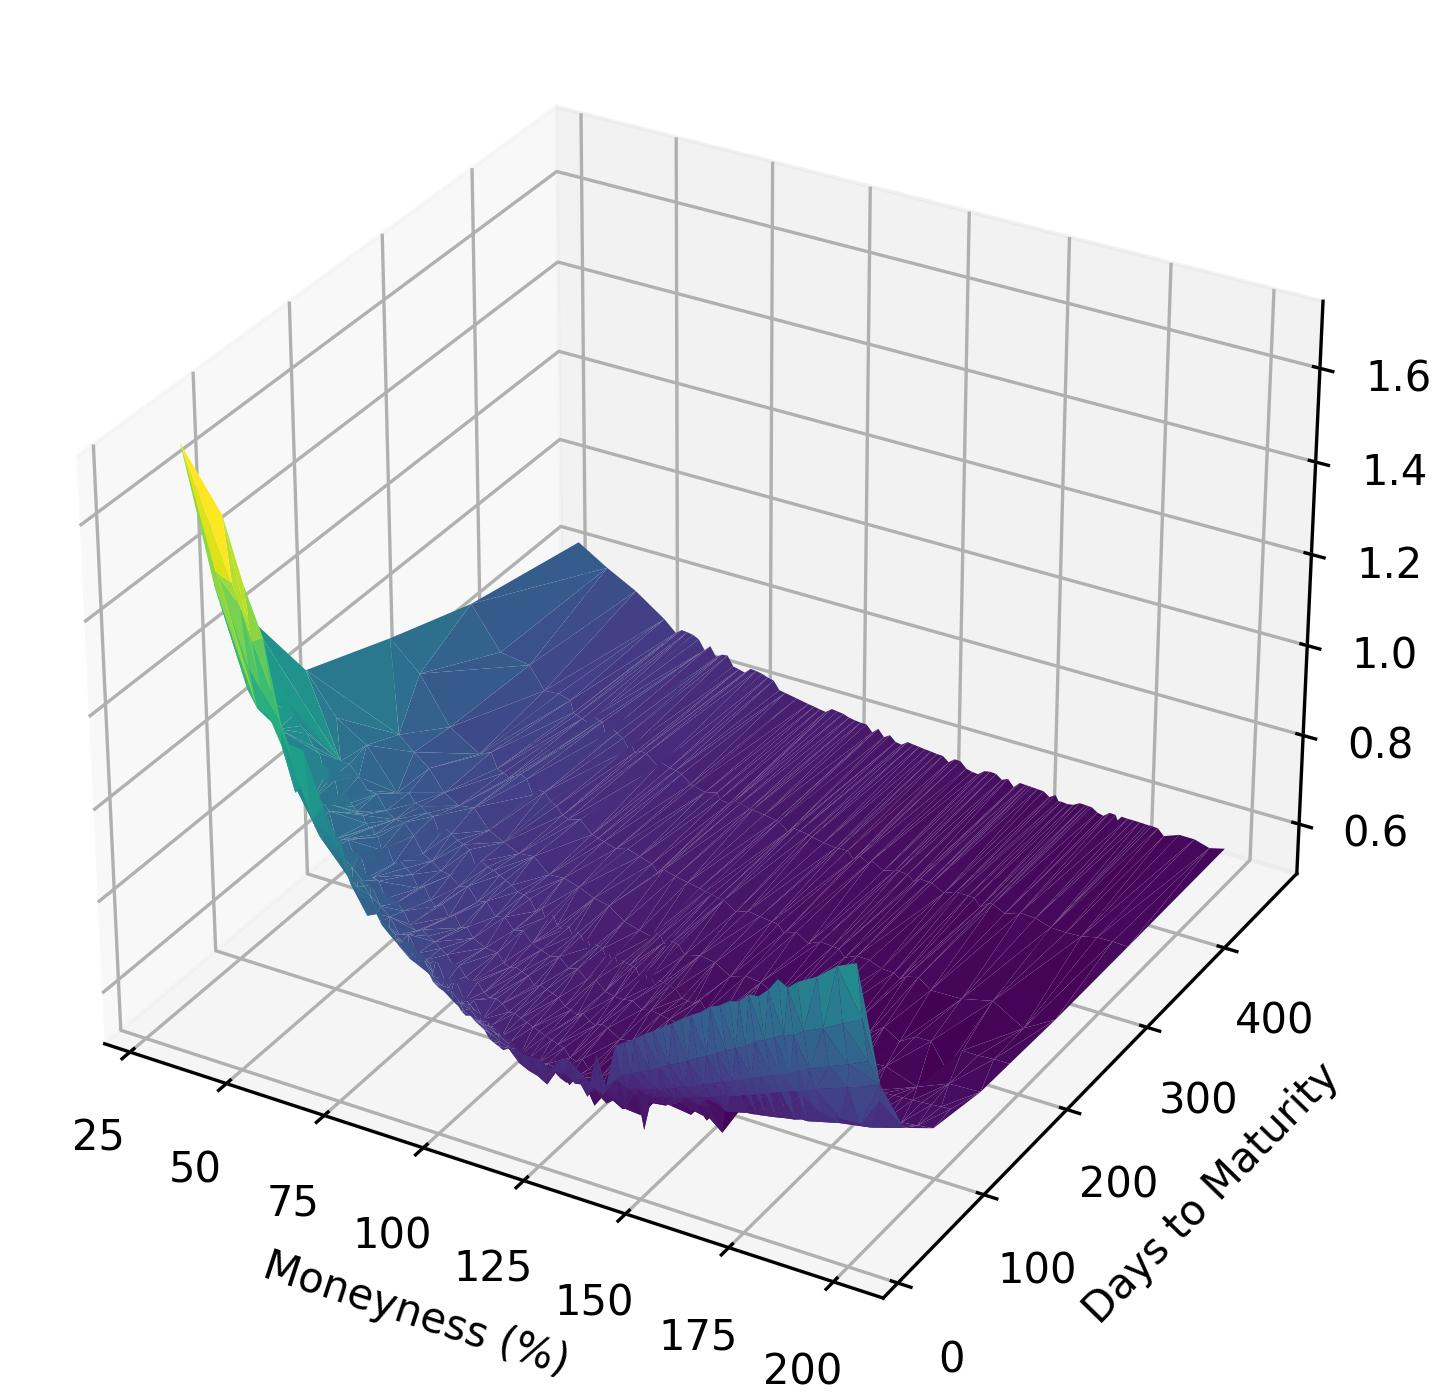
\includegraphics[width=0.5\linewidth]{TSLA_example_surface.jpeg}
  \caption{TSLA Implied Volatility Surface}
  \label{fig:sub1}
\end{subfigure}%
\begin{subfigure}{.5\textwidth}
  \centering
  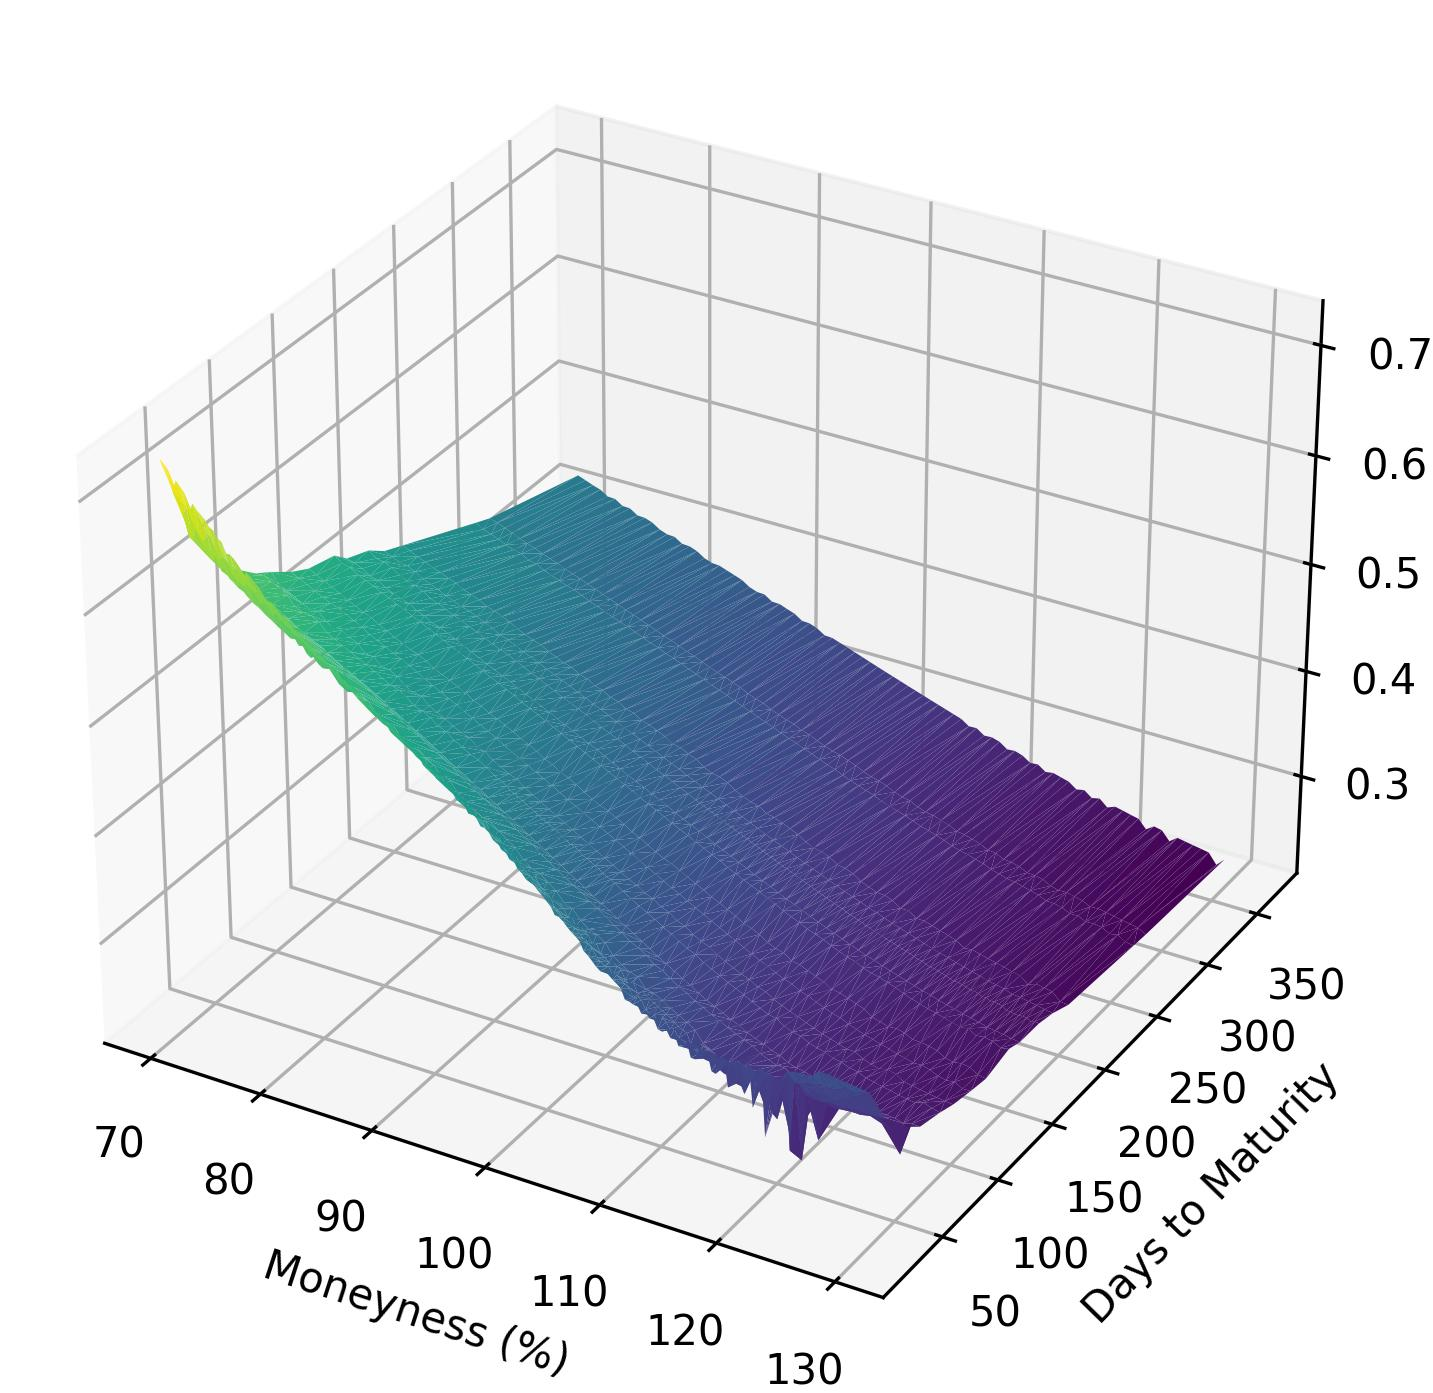
\includegraphics[width=0.5\linewidth]{NVDA.jpg}
  \caption{S\&P500 Implied Volatility Surface}
  \label{fig:sub2}
\end{subfigure}
\begin{subfigure}{.5\textwidth}
    \centering 
    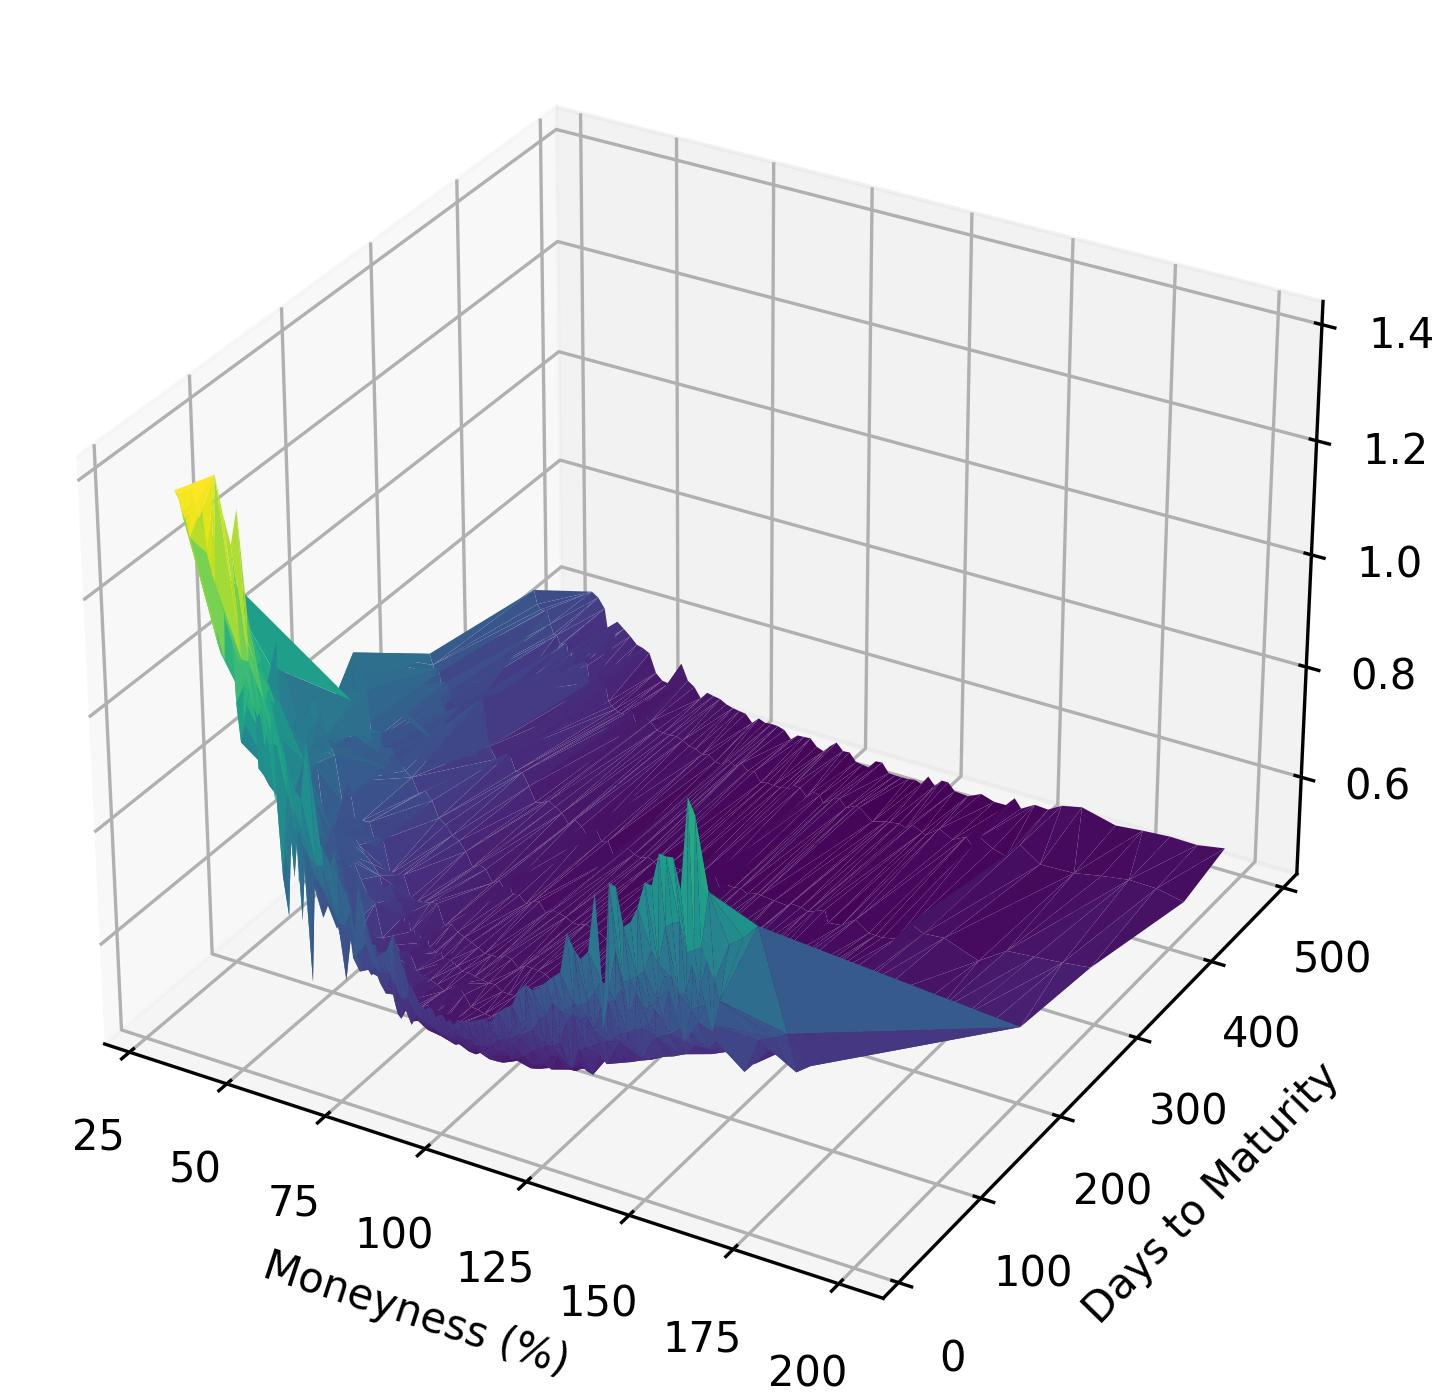
\includegraphics[width=0.5\linewidth]{SPX.jpg}
    \caption{NVDA Implied Volatility Surface}
    \label{fig:sub3}
\end{subfigure}
\caption{Example Implied Volatility Surfaces Used In Training and Testing}
\label{fig:test}
\end{figure}

\section{Model Architectures}

\subsection{Model Setup - Volatility Forecasting}
Our primary model architecture for forecasting volatility is a Multilayer Perceptron (MLP), which is specifically configured to handle the complexity and volume of our dataset effectively.

\subsubsection{Architecture Details}

Our MLP consists of four hidden layers each comprising 512 nodes, to forecast volatility. This architecture was chosen to effectively capture the complex patterns hidden within the large volumes of data. The use of both ReLU (Rectified Linear Unit) defined by \(\sigma(x) = max(0,x)\) and Leaky ReLU as activation functions introduces necessary non-linearities into the model, allowing it to learn and model the intricate dynamics of market volatility.

The MLP handles inputs through a large batch size of 4096, which not only improves computational efficiency but also stabilizes the learning updates during the training phase. Each input batch is processed through a network architecture where the input matrix \(X\), dimensioned at \(X \in \mathbb{R}^{4096\times5}\), interacts with a weight matrix \(W^{(1)}\) of dimensions \(W^{(1)} \in \mathbb{R}^{5\times512}\). This configuration outputs a matrix \(H\) of dimensions \(H \in \mathbb{R}^{4096\times512}\) through the operation:
 \(H = XW^{(1)}\), effectively mapping the high-dimensional data into a space where patterns can be more easily identified and learned.

\begin{figure}[H]
    \centering
    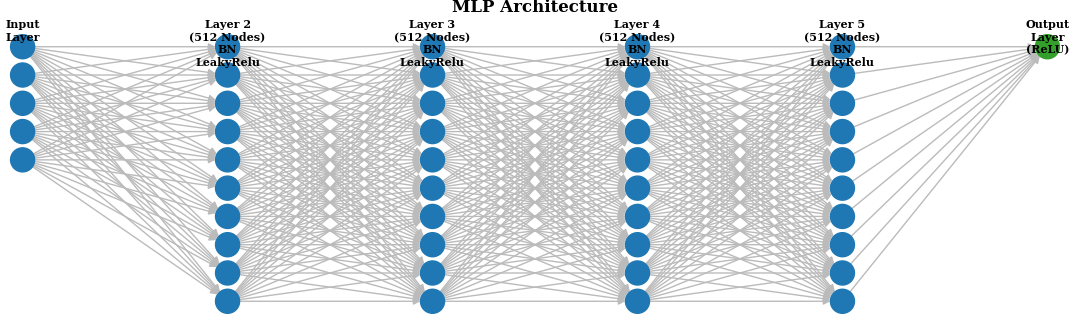
\includegraphics[width=0.85\linewidth]{MLP Architecture.png}
    \caption{MLP Architecture}
    \label{fig:enter-label}
\end{figure}



To enhance the stability and performance of our neural network, we implemented batch normalization following each hidden layer, as per the methodology introduced by Ioffe and Szegedy in 2015\cite{ioffe2015batch}. This normalization technique adjusts and scales the activations by normalizing the output of each layer using the equation:

\begin{equation}
    BN(x) = \gamma\cdot \frac{x - \hat{\mu}_B}{\hat{\sigma}_B} + \beta
\end{equation}

where \(B\) denotes a minibatch and \(x \in B\), \(\hat{\mu}_B\) and \(\hat{\sigma}_B\) denote the sample mean and standard deviations of the miniatch \(B\). \(\gamma\) and \(\beta\) are parameters learned during training. This process is crucial for reducing internal covariate shifts, thus speeding up the training process and reducing the model's overfitting tendency.

The model's performance is quantified using the Mean Squared Error (MSE) loss function, which calculates the average of the squares of the differences between the predicted values \(Y_i\) and the actual values \(\hat{Y_i}\):

\begin{equation}
    MSE = \frac{1}{N}\sum_{i=1}^{4096}(Y_i - \hat{Y_i})^2
\end{equation}

where \(Y_i\) is the \(i^th\) output generated by the neural network and \(\hat{Y_i}\) is the label corresponding to this set of features - the realized volatility for that option.

This loss function is particularly suited for regression problems like ours, where forecasting accuracy of continuous variables — such as volatility — is critical\cite{hodson2022root}.

\subsubsection{Comparative Models - Black-Scholes}
In our study, we benchmarked our results against a range of established baseline models. Given its extensive application in option pricing, the Black-Scholes model served as a natural reference point.

To evaluate the Black-Scholes model, we extracted the implied volatility from market prices using Brent's method, a hybrid root-finding algorithm that incorporates quadratic interpolation and the bisection method to narrow down the implied vol to a specific degree of accuracy\cite{brent1973some}. We specified the sensitivity to 1e-6 which gave us more than reasonable estimates for implied volatility. This method allowed us to more accurately compare the implied volatility derived from the market prices to the realized volatility used in our neural network. We then computed the mean squared error between the Black-Scholes implied volatility and the realized volatility:

\begin{equation}
    MSE = \frac{1}{4096}\sum_{i=1}^{4096} (\sigma_i^{realized} - \sigma_i^{implied})^2
\end{equation}


\subsubsection{Comparative Models - GARCH(1,1)}
As part of our comparative analysis, we included the GARCH(1,1) model\cite{bollerslev1986generalized}, a highly regarded univariate volatility forecasting model that has been extensively utilized in risk management. The GARCH(1,1) model is particularly favored for its ability to model financial time series that exhibit time-varying volatility, an aspect crucial in the accurate prediction of financial market behaviors.

The operational equation for the GARCH(1,1) process is defined as:

\begin{equation}
    \sigma_t^2 = \omega + \alpha r_{t-1}^2 + \beta_{t-1}^2
\end{equation}
with \(\omega \geq 0, \hspace{0.2cm}\alpha \geq 0, \hspace{0.2cm} \beta \geq 0\), and at least one of these inequalities being strict.

\(\sigma^2_t\) denotes the conditional variance at time \(t\), \(r^2_{t-1}\) is the squared returns from the previous period, \(\omega, \alpha, \and \beta\) are parameters to be estimated with \(\omega \geq 0\), \(\alpha \geq 0\), and \(\beta \geq 0\) ensuring that at least one of these inequalities is strict. The parameters \(\alpha\) and \(\beta\) are crucial as they measure the response of volatility to market movements (news impact) and the persistence of volatility (volatility clustering) respectively. 

We evaluated the performance of the GARCH(1,1) model in the context of our dataset by analyzing its ability to forecast next-period volatility accurately. This was done by computing the Mean Squared Error (MSE) between the predicted volatility and the realized volatility of the market.


\subsection{Model Setup - Volatility Surface Classification}
\subsubsection{Motivation}
We felt that an inadequate amount of research was done on looking at company/industry-specific trends in the volatility surface. Thus, we decided that if we were able to train a neural network to classify a given volatility surface into a sector, or even predict the correct underlying stock to which the surface belonged, this could be evidence to suggest that implied volatility dynamics are, in fact, unique to every stock. 

We knew that a trained human eye could easily distinguish between an index and an equity option, due to the distinct characteristics of the volatility 'skew'\cite{xing2010does}. Index options have high 'downside skew', driven by demand for downside protection inflating out-of-the-money put option prices and the fact that volatility increases when the market falls, but low 'upside skew', since there is not as much demand for index upside, especially further out-of-the-money since indices do not rally to the same degree that a single name stock does\cite{ang2006cross}. This leads to the index 'volatility smirk'. Conversely, single-name equity options have both high downside skew and high upside skew, because people like to speculate on rapid price appreciation, and this leads to the equity 'volatility smile'. We realized that, ultimately, the implied volatility surface is the representation of the market's expectation for price movement. Thus, volatility dynamics should be relatively unique to each sector and maybe even each stock. 

\subsubsection{Architecture Details}
For this section, we built three Convolutional Neural Networks. Sector and individual classification structures featured three convolutional layers, with each one followed by batch normalization and a ReLU activation function, with max pooling applied after activation. The networks start with three input channels (RGB compatible), and the number of filters increases from 32 in the first layer, 64 in the second and 128 in the final layer. Convolutional layers use a kernel of size 3, a stride of 1 and padding of 1. After passing through the convolutional stages, the output is flattened and processed through two fully connected layers. The first dense layer has 512 units, and the second (the output layer) varies between 5 (sector classification) and 18 (underlying classification) units, depending on which classification the model is doing. The index vs equity model was simpler as it was a binary classification task, so there was one less convolutional layer and fewer filters, but still used ReLU and max pooling.

\begin{figure}[H]
    \centering
    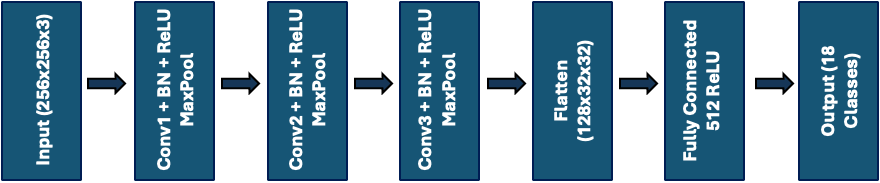
\includegraphics[width=0.5\linewidth]{cnn box.png}
    \caption{18 Output Class CNN Architecture}
    \label{fig:enter-label}
\end{figure}

\section{Results and Discussion}

\subsection{Volatility forecasting}
 Much of the hyperparameter optimization concerned finding optimal learning rates and did not necessitate any regularization methods. We found out early on in our testing that implementing weight decay and dropouts led to worse performance and unstable convergence so we opted to exclude these. We also settled on using the Adam Optimizer which yielded greater accuracy as opposed to SGD or other Adam family optimizers (eg. AdamW, Adagrad). Similarly to how was performed in the Stanford Paper, we looked at iteratively adjusting the learning rate, to prevent overfitting and allow steady convergence. We found that a learning rate of 4e-5 for 10 epochs, followed by 3e-5 for 20 epochs gave us the highest accuracy and the least overfitting.

Having established an optimal hyperparameter setup for our Neural Network, we compared performance statistics to the baseline models. We found that the MLP converged after 30 epochs and returned an average mean-squared error of 0.004821 with greater fluctuations in validation loss in subsequent epochs. Our Black Scholes model performed the worst out of the 3, with a Mean-squared error of 0.1304 on a batch size of 4096. Finally, the GARCH(1,1) model performed very well, yielding a mean-squared error of 0.007645 on a batch size of 4096. 

Below is a sample of the predicted vs realized volatility of the 3 models. 

\begin{figure}[H]
\centering
\begin{subfigure}{.5\textwidth}
  \centering
  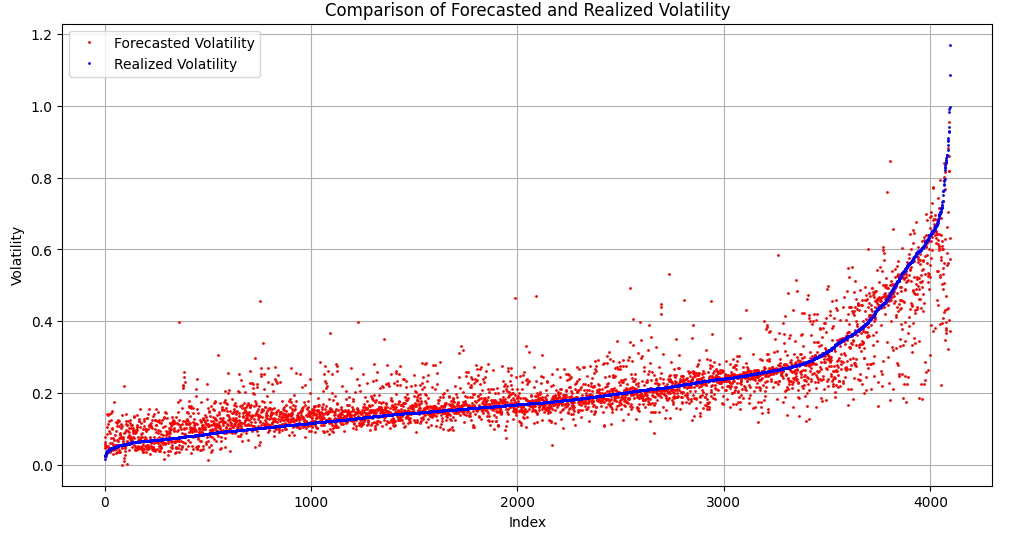
\includegraphics[width=0.6\linewidth]{MLP2-4-3e-5-30epochs.png}
  \caption{Predicted vs Realized volatility - MLP}
  \label{fig:sub1}
\end{subfigure}%
\begin{subfigure}{.5\textwidth}
  \centering
  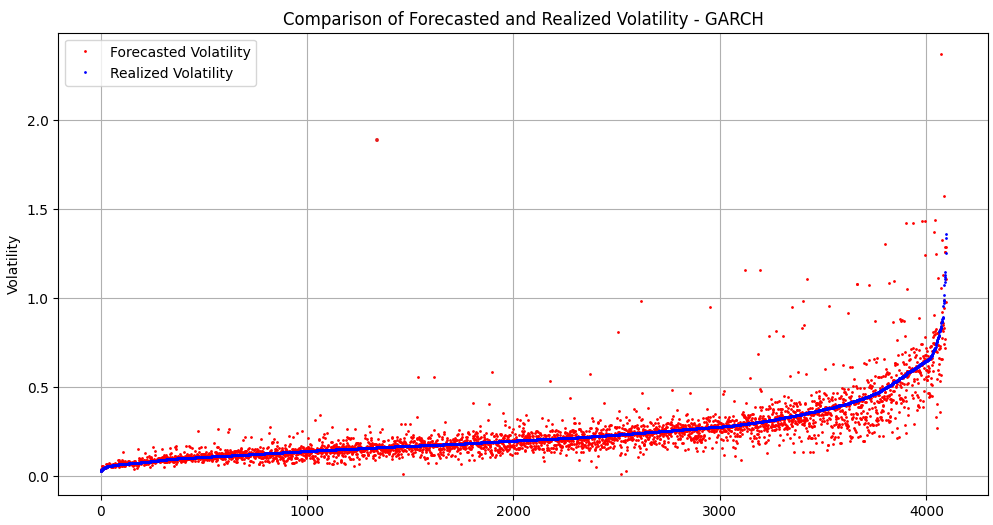
\includegraphics[width=0.6\linewidth]{GARCH(1,1).png}
  \caption{Predicted vs Realized volatility - GARCH(1,1)}
  \label{fig:sub2}
\end{subfigure}
\begin{subfigure}{.5\textwidth}
    \centering 
    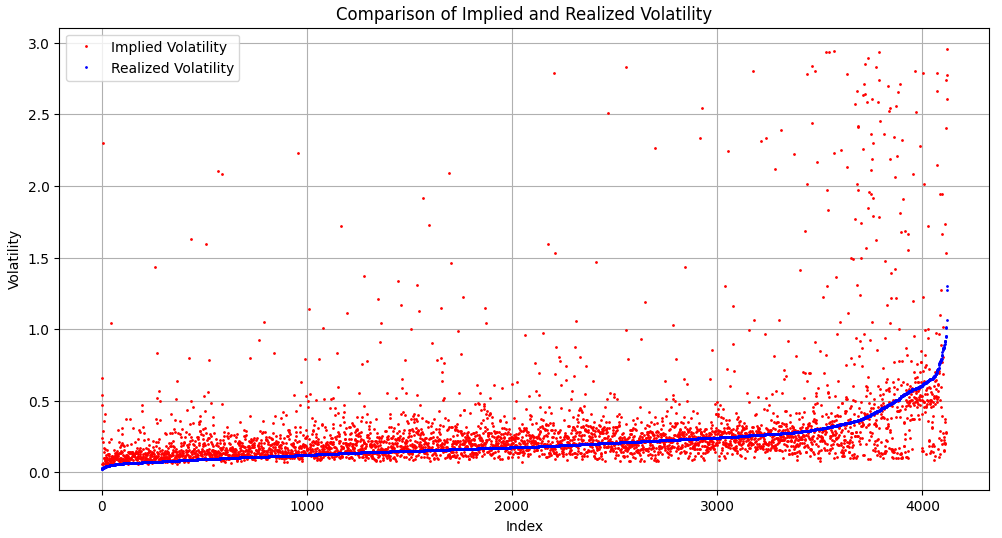
\includegraphics[width=0.6\linewidth]{Black-Scholes.png}
    \caption{Implied Volatility vs Realized volatility - Black-Scholes}
    \label{fig:sub3}
\end{subfigure}
\caption{MLP vs Benchmark Models Performance}
\label{fig:test}
\end{figure}

As we can see, the model with the tightest spread between realized and predicted volatility was the MLP. It might not immediately be apparent, but looking at the y-axis scale of the plots we can see that GARCH had a greater spread. 

\subsection{Volatility Surface Classification}
Overall, the models performed extremely well given the nature of what they had to classify. For sector and individual classification, we found that a 32-batch size was best, with a starting learning rate of 0.001 using the AdamW optimizer. We used early stopping to help us identify after how many epochs validation loss started to exhibit overfitting and found that 14 epochs were optimal. We found that utilising a learning rate scheduler with a gamma of 0.5 and step size 10 greatly improved the accuracy in the final 4 epochs.

The index vs equity binary classification task was the best, with 100\% training, validation and testing accuracy after 5 epochs. We expected high performance given that when looking at the data, it is quite obvious which surfaces belong to index options due to several very distinct features. The confusion matrix for this model indicated that all 1,980 unseen test images were correctly classified. 

The sector classification model had a training accuracy of 98.77\% and a testing accuracy of 90.31\%. We excluded index options in this dataset. The very high level of accuracy observed in testing confirms the fact that implied volatility is unique to sectors, although not necessarily to the human eye. Training accuracy after the first epoch was only 46\%. We were able to deploy efficient hyperparameter optimization to achieve a final accuracy of 98.7\% after 14 epochs and no signs of overfitting.


\subsubsection{Individual Underlying Classification}

The CNN's job now becomes much more difficult as it can no longer rely on the distinct index volatility smirk to classify for 15 of the output classes. This is reflected in the lower accuracy, yet it was still surprisingly high. The individual underlying classification model achieved a training accuracy of 90.45\%, a validation accuracy of 78.06\%, and a testing accuracy of 78.23\%. There were some slight signs of overfitting on the validation loss around epoch 8, but the learning rate scheduler did a great job at stabilising this after epoch 10. The table below shows the per-class accuracy of the model.

\begin{tabular}[H]{ |p{1.03cm}|p{1.03cm}|p{1.25cm}||p{1.03cm}|p{1.03cm}|p{1.25cm}||p{1.03cm}|p{1.03cm}|p{1.25cm}|  }
 \hline
 \multicolumn{9}{|c|}{Per-Class Accuracy} \\
 \hline
 Ticker & Label & Accuracy & Ticker & Label & Accuracy & Ticker & Label & Accuracy\\
 \hline
 BAC & 0 & 77.8\% & META & 6 & 75.7\% & RUT & 12 & 92.8\%\\
 CVX & 1 & 82.2\% & MRNA & 7 & 71.0\% & SPX & 13 & 96.4\% \\
 ENB & 2 & 89.4\% & MS & 8 & 70.64\% & TSLA & 14 & 89.3\%\\
 JNJ & 3 & 87.9\% & NDX & 9 & 62.8\% & UL & 15 & 79.7\%\\
 JPM & 4 & 70.0\% & NVDA & 10 & 81.7\% & WMT & 16 & 46.9\%\\
 KO & 5 & 93.2\% & PFE & 11 & 85.5\% & XOM & 17 & 53.7\% \\
 \hline
\end{tabular}

The most standout result was the fact that the most liquid options (e.g. SPX, TSLA, RUT) had the best test accuracy, with SPX taking the top spot. We think this is due to the fact that there was much cleaner data for these underlying assets as a result of their superior liquidity. This also holds on the opposite end of the spectrum, with more illiquid energy and consumer stock options such as XOM and WMT dominating the bottom. The big outliers are NDX (Nasdaq), KO (Coca-Cola) and ENB (Enbridge). The confusion matrix below shows that NDX was classified as one of the other two index options 62 times, which is understandable as indices are very similar. As for KO and ENB, we think that these options are so illiquid that the lack of data had large distortion impacts on the volatility surfaces, which helped the model easily tell them apart.



\begin{figure}[H]
\centering
\begin{subfigure}{.5\textwidth}
  \centering
  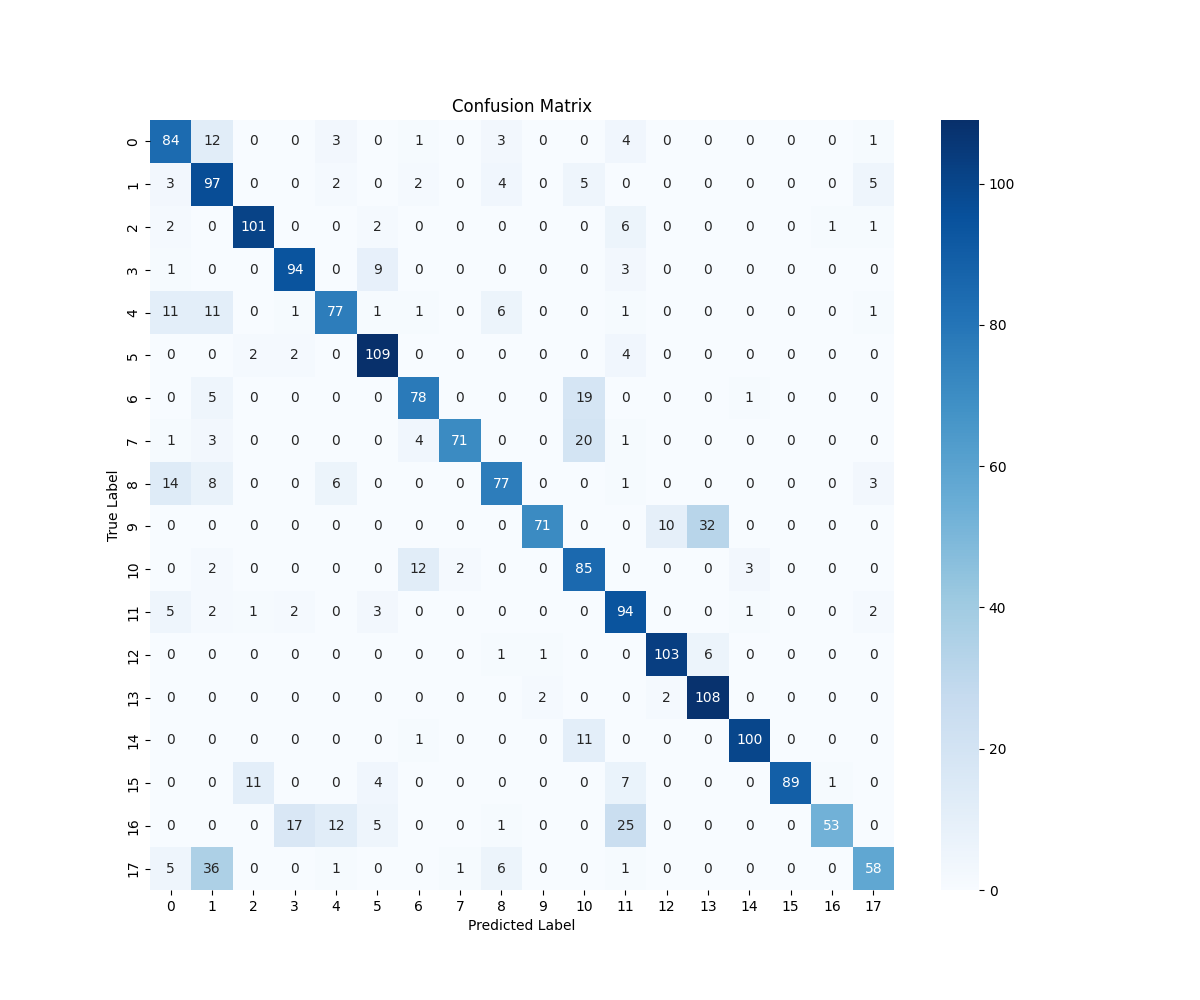
\includegraphics[width=1\linewidth]{Confusion_Matrix_REAL.png}
  \caption{Individual Underlying Classification}
  \label{fig:sub1}
\end{subfigure}%
\begin{subfigure}{.5\textwidth}
  \centering
  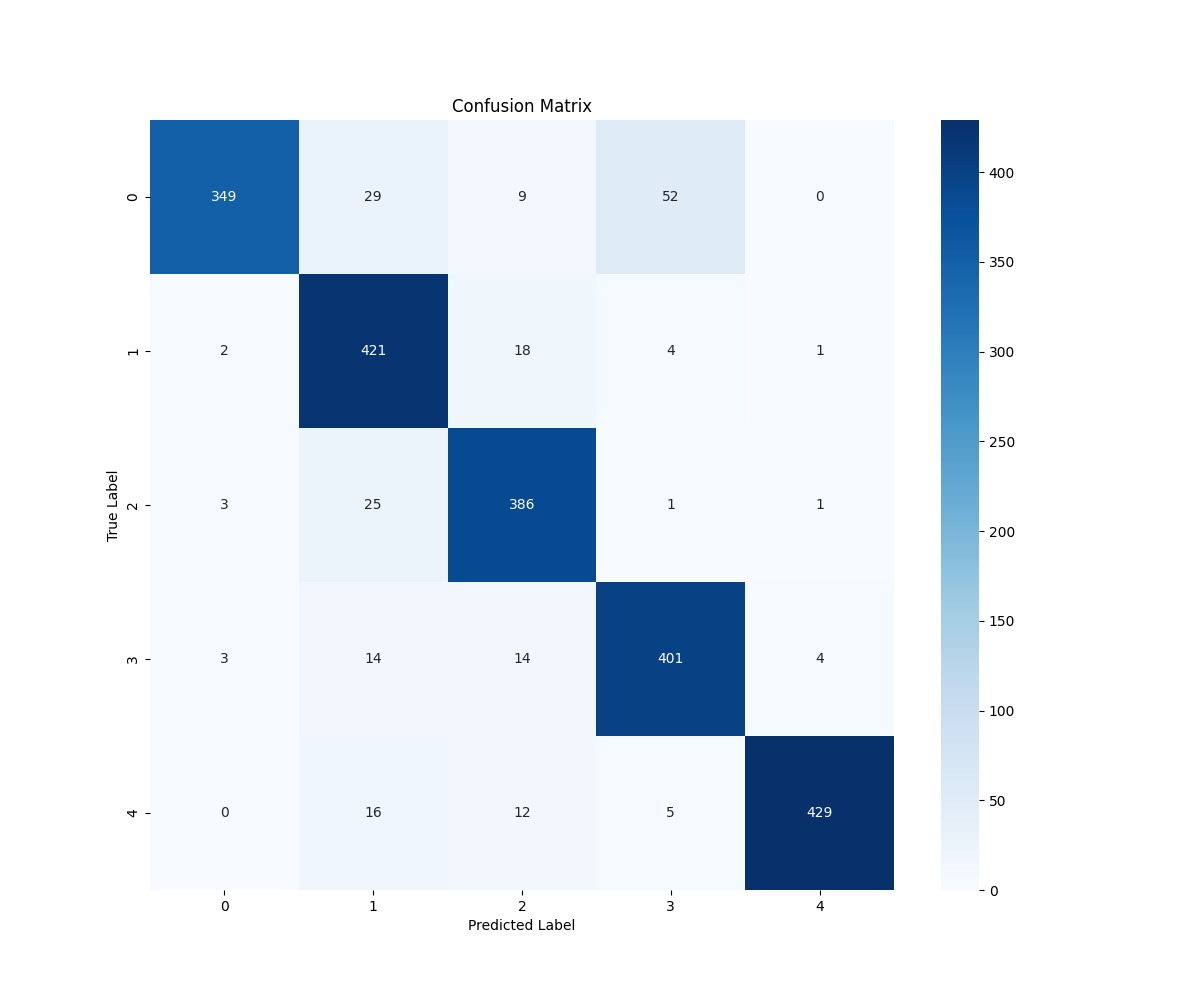
\includegraphics[width=1\linewidth]{Confusion matrix 2.jpg}
  \caption{Sector Classification}
  \label{fig:sub2}
\end{subfigure}
\end{figure}

\section{Conclusion}

Our research has demonstrated the substantial capabilities of deep neural networks (DNNs) in accurately modeling and forecasting volatility in financial markets. By integrating inputs traditionally used in the Black-Scholes model, our DNNs were not only able to predict realized volatility with high accuracy but also uncover consistent dislocations between implied and realized volatility. The fact that Black-Scholes implied volatility is, on average, overpriced, is likely due to supply and demand dynamics, recently exacerbated by retail-driven options volatility dislocation (retail traders hyping up popular stocks such as Tesla). Our model excels in avoiding these dynamics, using advanced neural network parameters to decode and predict the nuances of volatility. 

Overall, our implied volatility surface classification models performed extremely well and highlighted some interesting observations. Firstly, we showed index options can very easily be distinguished from equity options. This was not a large surprise to us.

Secondly, we saw that liquidity played a very important role in classification accuracy. Of all the stocks we classified, the tech stocks were individually classified correctly more than most of the other underlying assets (excluding index options, which are even more liquid, and one or two outliers). The less liquid options (energy stocks, consumer stocks, etc) were typically classified with significantly lower accuracy. The less liquid, the (usually) less accurate the classification. We think this is due to two things: data distortion and market forces. Less liquid options tended to have worse quality data (i.e. missing implied volatility values for some expiries), which sometimes distorted the volatility surface images we generated. This likely made it harder for our CNNs to learn the distinct features of the surfaces and hence cause the model to have trouble distinguishing between stocks. The data distortion is likely the reason why the energy sector was the best classified with 94.4\% testing accuracy, highlighting a significant weakness in our model and data, since the reason for outperformance was not caused by unique volatility but poor data as the model learned the data distortions. However, we also believe market forces have an impact, given that less liquid options typically might have more similar volatility surfaces because the uniqueness on a surface is generated by demand and supply on the constituent option contracts in the surface. This would explain why TSLA and NVDA were classified so well - because the market actually expresses more of a view on these stocks as they are simply more interesting in their price dynamics. In conclusion, however, our three CNNs were very capable in classifying volatility surfaces into sectors, underlying names, and indices vs equities. While proposed more as a way to provide evidence for volatility uniqueness across stocks, potential applications in the real world could include using a better trained CNN to identify deviations from the normal shape of the implied volatility surface in order to monetize mean reversion.

To improve this project, we would suggest a few things. Firstly, expanding the dataset (especially for the classification task). While our 13,000 images were sufficient, more data is always better. Unfortunately, we were limited by computational resources, which also hindered our ability to optimize hyperparameters to the fullest extent as well as interpolating risk free rates perfectly for the forecasting task. There is also so much more we could explore in the forecasting model: potentially using an LSTM model, or most interestingly increasing the range of input parameters such as historical volatility, trading volume, option volume imbalance and open interest. We strongly believe this could increase the predictive performance of the model.

We hope that this research proved insightful not only in uncovering persistent trends in volatility but also in establishing the utility and scope of Artificial Neural Networks for Financial Analysis and Risk Management. We believe that the applications of AI to the securities markets are immense, given that most risk systems are yet to incorporate neural networks, and should prove to be very useful for sell-side investment banks and other market makers in more efficient hedging and risk management.



\vspace{13cm}
\section{References}

\bibliographystyle{plain}
\bibliography{references}

\section{Code for Volatility Forecasting (Hyperlinks):}

\begin{itemize}
  \item \href{https://colab.research.google.com/drive/1HeMWjGCQj-xAVBxnDBg6qXo_OX-pYAs1?usp=sharing}{Data Preprocessing Checkpoint 1}
  \item \href{https://colab.research.google.com/drive/1u55O96Ta_LaE7qLtDCZf6g8zyA8UWPO9?usp=sharing}{Data Preprocessing Checkpoint 2}
  \item \href{https://colab.research.google.com/drive/1MKXJ33bUN4k-Ffge3MftOQZNgDVGqW_h?usp=sharing}{Data Preprocessing Checkpoint 3}
  \item \href{https://colab.research.google.com/drive/13x2EyBgopebi3oArXLRMYQGjUKCbo3L3?usp=sharing}{Data Preprocessing Checkpoint 4}
  \item \href{https://colab.research.google.com/drive/1zWTs-i5BKwGLTYSMLkmfqr1Rj4KSEpsy?usp=sharing}{Data Preprocessing Checkpoint 5}
  \item \href{https://colab.research.google.com/drive/1pWdwa8RfqfbnQH-5V2prGx3wMbhMlESW?usp=sharing}{Data Preprocessing Checkpoint 6}
  \item \href{https://colab.research.google.com/drive/1HgYntz5i6Q6S4bpY8tXiFTjAV7C7cp-f?usp=sharing}{Data Preprocessing Checkpoint 7}
  \item \href{https://colab.research.google.com/drive/12KdD33w15luj7t9wdnv57r-9qA8yA34Q?usp=sharingQ}{Data Preprocessing - Black-Scholes Model}
  \item \href{https://colab.research.google.com/drive/1TxcJYcpTQzVPnckIWfbtmfqlK8NBn2Pz?usp=sharing}{Data Preprocessing - Black-Scholes model on Individual Securities}
  \item \href{https://colab.research.google.com/drive/191OuoTBpQzLO_Xz8Bwu8HpFzU-NgTBin?usp=sharing}{Baseline Models - GARCH(1,1)}
  \item \href{https://colab.research.google.com/drive/1-NfN8dnuTuVX1NxqwJdX2o-P0r6aM7Bd?usp=sharing}{Baseline Models - Black-Scholes}
  \item \href{https://colab.research.google.com/drive/1RDi-4RopwcRBYp094BoeJEAYtcHtuHxS?usp=sharing}{MLP Model for Call Options}
  \item \href{https://colab.research.google.com/drive/1UQmmsksDU6tx8cm-BMsMiWxZ-HXJ6s7k?usp=sharing}{MLP Model for Put Options}
  \item \href{https://colab.research.google.com/drive/1nzuaynHSq1otJmYJ0GmhK8pzl7CqCLQb?usp=sharing}{Results Plots}  
\end{itemize}

\section{Code for Volatility Surface Classification (Hyperlinks):}

\begin{itemize}
  \item \href{https://colab.research.google.com/drive/1RPZpqyt33PQb9ZkAlst8CjZph5h1zgBK?usp=sharing}{Data Preprocessing Initial Testing and Exploration}
  \item \href{https://colab.research.google.com/drive/1PO-9FZiYK0rzfPjc7jJBSP_qxUhoOPxs?usp=sharing}{Data Preprocessing - Extracting Equity Implied Volatility Surfaces}
  \item \href{https://colab.research.google.com/drive/1moMm0MVd46vPRBijcpB2r7ZE3xOhrWAT?usp=sharing}{Data Preprocessing - Extracting Index Implied Volatility Surfaces}
  \item \href{https://colab.research.google.com/drive/128uu0wZXvBpfcqyY2Le41YxMySnyBIXk?usp=sharing}{Model 1 - Index vs Equity Option Classifier}
  \item \href{https://colab.research.google.com/drive/1e-zCuNWVzXSWbTsUch87-hY_tp_T7Boy?usp=sharing}{Model 2 - Sector Classification}
  \item \href{https://colab.research.google.com/drive/16w8rRRtv4U_B2WVU_WHdnCJxcheVtrpB?usp=sharing}{Model 3 - Individual Underlying Classification}
\end{itemize}

\section{Statement on Contributions}

Both group members contributed equally to this project with a 50/50 split.

\end{document}
